%% Einbinden in Trigo: Rechtwinkliges Dreieck, aber auch
%% in Planimetrie: Satz des Pythagoras
%%
%% Hier:
%%   * Allgemeine Form
%%   * Höhensatz
%%   Nicht dabei:
%5     -Sinus/Cosinus/Tangens (dies ist nur in Trigo)
%5     -Höhensatz (der kommt nur bei der Planimetrie)


\section{Rechtwinkliges Dreieck}\index{Dreieck!rechtwinkliges}\index{rechtwinkliges Dreieck}
\sectuntertitel{... nein, wir sind nicht Asterix und Obelix: Wir sind
  Römer, wir sind Sinus und Cosinus ...\footnote{S. Asterix -- Tour de France -- Seite 40}}

%%\GESOTadBAlgebra ????
%%%%%%%%%%%%%%%%%%%%%%%%%%%%%%%%%%%%%%%%%%%%%%%%%%%%%%%%%%%%%%%%%%%%%%%%%%%%%%%%%
\subsection*{Lernziele}

\begin{itemize}
 \item Satz des Pythagoras Formel
 \item Höhensatz
 \item sinus/cosinus/tangens
\end{itemize}

\TALSTadBMTG{28}{2.3}



%% Load this only once (the first occurence)!
%% see here: https://tex.stackexchange.com/questions/195157/is-there-any-analog-to-pragma-once-in-latex
%%\ifcsname XX_Pythagoras.tex\endcsname
%%  \expandafter\endinput
%%\fi
%%\expandafter\gdef\csname XX_Pythagoras.tex\endcsname{loaded}



%%%%%%%%%%%%%%%%%%%%%%%%%%%%%%%%%%%%%%%%%%%%%%%%%%
\newpage

\subsection{Rechtwinkliges Dreieck}

\definecolor{qqwuqq}{rgb}{0,0.39,0}
\definecolor{xdxdff}{rgb}{0.49,0.49,1}
\definecolor{qqqqff}{rgb}{0,0,1}
\begin{tikzpicture}[line cap=round,line join=round,>=triangle 45,x=1.0cm,y=1.0cm]
\clip(-0.54,0.17) rectangle (5.83,4.51);
\draw [shift={(3.35,3.58)},color=qqwuqq,fill=qqwuqq,fill opacity=0.1] (0,0) -- (-154.75:0.95) arc (-154.75:-64.75:0.95) -- cycle;
\draw (0,2)-- (4.56,1.02);
\draw (0,2)-- (3.35,3.58);
\draw (3.35,3.58)-- (4.56,1.02);
\fill[color=qqwuqq,fill=qqwuqq,fill opacity=0.1] (3.16,3.05) circle (0.03);
\begin{scriptsize}
\fill [color=qqqqff] (0,2) circle (1.5pt);
\draw[color=qqqqff] (0.25,2.42) node {$A$};
\fill [color=qqqqff] (4.56,1.02) circle (1.5pt);
\draw[color=qqqqff] (4.81,1.44) node {$B$};
\fill [color=xdxdff] (3.35,3.58) circle (1.5pt);
\draw[color=xdxdff] (3.61,4.01) node {$C$};
\draw[color=qqwuqq] (2.37,2.49) node {$90\textrm{\degre}$};
\end{scriptsize}
\end{tikzpicture}

\begin{definition}{Rechtwinkliges Dreieck}{}
Im \textbf{rechtwinkligen} Dreieck misst der Winkel gegenüber der
längsten Seite 90\degre.
\end{definition}



\subsection{Satz des Pythagoras (Repetition)}\index{Pythagoras!Trigonometrie}\index{Satz des Pythagoras!Trigonometrie}
\label{satzDesPythagoras}
\begin{gesetz}{Satz des Pythagoras}{}
Im rechtwinkligen Dreieck mit Hypotenuse $c$ gilt:
$$a^2 + b^2 = c^2$$
\end{gesetz}

\TNTeop{Platz für graphischen Beweis\vspace{3cm}}



%%%%%%%%%%%%%%%%%%%%%%%%%%%%%%%%%%%%%%%%%%%%55
\subsection{Höhensatz (optional)}\index{Höhensatz}

Im rechtwinkligen Dreieck mit Hypotenusenabschnitten $p$ und $q$ gilt:
$$h^2=p\cdot{}q$$

Beweise:

\TNT{6.4}{

Beweis mit Ähnlichkeit: $p:h = h:q$, somit folgt der Satz direkt.

Optional: Beweis mit Pythagoras: $h^2 = a^2 - p^2$ und $h^2 = b^2 -
  q^2$.\\
Somit gilt
$2h^2 = a^2 + b^2 - p^2 - q^2 = c^2 - p^2 - q^2 = (p+q)^2 -p^2 - q^2 =
  p^2 +2pq + q^2 - p^2 - q^2 = 2pq$\\
Daraus folgt:$$h^2=pq.$$
}

\subsection*{Aufgaben}
\AadBMTG{37}{8., 9., 11., 12., 13., 15., 28., 29., 30.}

\newpage

\subsection{Spezielle Dreiecke}\index{Dreiecke!spezielle}\label{spezielleDreiecke}

\subsubsection*{Lernziele}
\begin{itemize}
  \item 45\degre: Das halbe Quadrat\index{Quadrat}
  \item 30\degre/60\degre: Das halbe gleichseitige
  Dreieck\index{Dreieck!gleichseitiges}\index{gleichseitiges Dreieck}
\end{itemize}

\TadBMTG{33}{2.4.1}



\begin{samepage}
\subsection{gleichseitiges Dreieck und halbes Quadrat}\index{Dreieck!gleichseitiges}\index{gleichseitiges Dreieck}\index{Quadrat!Diagonale}\index{halbes Quadrat}

%%\renewcommand{\arraystretch}{2.4}
\begin{bbwFillInTabular}{|c|p{5cm}|} 
  \hline
  \raisebox{-18mm}{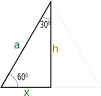
\includegraphics[width=4cm]{tals/plani/img/gleichseitigesDreieck.png}} &
  $\begin{array}{ll}
    x=& \frac{a}{2}                     \\
    h=& \sqrt{3}\cdot{}x                \\
    h=& \frac{\sqrt{3}}{2}\cdot{}a
  \end{array}$ \\

  \hline
  \raisebox{-24mm}{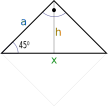
\includegraphics[width=5cm]{tals/plani/img/halbesQuadrat.png}} &
  $\begin{array}{ll}
    x=& \sqrt{2}\cdot{}a            \\
    h=& \frac{x}{2}                 \\
    h=& \frac{\sqrt{2}}{2} \cdot{} a\\
    a=& \sqrt{2}\cdot{}h
  \end{array}$ 
  \\
  
  \hline
\end{bbwFillInTabular} 

Beweis: Aufg. 19. und 20. \cite{marthaler20geom}

%%\TALS{Siehe auch \cite{frommenwiler18geom} S. 25 Kapitel 1.2.2}

\end{samepage}



\subsection*{Aufgaben}
\AadBMTG{37}{7., 19., 20., 21., 24., 26., 33., 34., 40. und 41. }
\newpage
